\section{Eve}\label{eve}

\subsection{Namapování dat z~pohledů na zdroje}\label{namapovuxe1nuxed-dat-z-pohledux16f-na-zdroje}

Ve výchozím stavu Eve předpokládá uložení dat v~NoSQL databázi MongoDB. Je možné si napsat vlastní správce dat, ale jednodušší je použít již existující modul \verb!eve-sqlalchemy!. Pro namapování dat je třeba popsat jednotlivé zdroje pomocí SQLAlchemy modelů a poté je zaregistrovat.

\protect\hyperlink{code:eve:mapping}{V~ukázce} můžete vidět příklad modelu pro kurzy i vlastní dekorátor pro jeho registraci. Funkce \verb!registerSchema()! z~\verb!eve-sqlalchemy! vygeneruje pro každý model schéma, které je následně možné upravit.

Je třeba zdůraznit, že Eve očekává primární klíče pojmenované ve tvaru \emph{\_id}, což sice umožňuje změnit, ale pouze globálně (například zde v~ukázce na \emph{id}); proto již je položka \emph{id\_subjects} přejmenována na \emph{id}, ačkoli o~přejmenování položek bude řeč až dále.

\begin{listing}[htbp]
\caption{{\label{code:eve:mapping}Eve: Namapování dat z~pohledů na zdroje}}
\begin{minted}[bgcolor=codebg]{python}
domain = {}
config.ID_FIELD = config.ITEM_LOOKUP_FIELD = 'id'


def register(cls):
    '''Decorator that registers it and keeps track of it'''
    plural = cls.__name__.lower() + 's'
    registerSchema(plural)(cls)
    domain[plural] = cls._eve_schema[plural]

    # make sure id is our id_field
    # IMHO this should happen automatically but it doesn't
    domain[plural]['id_field'] = config.ID_FIELD

    # make all ids of type objectid
    # should not be necceassry, but feels good :)
    domain[plural]['schema']['id']['type'] = 'objectid'

    return cls

@register
class Course(Base):
    __tablename__ = 'v_subjects'

    id = Column('id_subjects', Integer,
                primary_key=True)
    shortcut = Column(String)
    day = Column(Integer)
    begin = Column(String)
    end = Column(String)
    notice = Column(String)
    semester = Column(Integer)
    sport = Column(Integer, ForeignKey('v_sports.id_sport'))
    hall = Column(Integer, ForeignKey('v_hall.id_hall'))
    lector = Column(Integer, ForeignKey('v_lectors.id_lector'))


SETTINGS = {
    # ...
    'DOMAIN': domain,
}

app = Eve(settings=SETTINGS)
\end{minted}
\end{listing}

Namapování dat z~pohledů na zdroje v~Eve je možné, systematické a jednoduché.

\subsection{Přejmenování položek}\label{pux159ejmenovuxe1nuxed-poloux17eek}

Jak můžete vidět \protect\hyperlink{code:eve:rename}{v~ukázce}, pro přejmenování položek stačí provést jednoduchou úpravu modelu -- přejmenovat třídní atributy a poskytnout konstruktoru \verb!Column! název sloupce jako první argument.

\begin{listing}[htbp]
\caption{{\label{code:eve:rename}Eve: Přejmenování položek}}
\begin{minted}[bgcolor=codebg]{python}
@register
class Teacher(Base):
    __tablename__ = 'v_lectors'

    id = Column('id_lector', Integer, primary_key=True)
    degrees_before = Column('title_before', String)
    first_name = Column('name', String)
    last_name = Column('surname', String)
    degrees_after = Column('title_behind', String)
    personal_number = Column('pers_number', Integer)
    url = Column(String)
\end{minted}
\end{listing}

Přejmenování položek v~Eve je možné, systematické a triviální.

\subsection{Prolinkování zdrojů ve stylu HATEOAS}\label{prolinkovuxe1nuxed-zdrojux16f-ve-stylu-hateoas}

Eve se dozví o~relacích mezi objekty ze schématu. Protože automaticky vytvořené schéma není dostatečné, je třeba jej mírně upravit. Toho jsem docílil úpravou v~dekorátoru \verb!@register!, kterou můžete vidět \protect\hyperlink{code:eve:links1}{v~ukázce}.

\begin{listing}[htbp]
\caption{{\label{code:eve:links1}Eve: Úprava schématu}}
\begin{minted}[bgcolor=codebg]{python}
def register(cls):
    # ...

    # change data_relation's schema a bit
    for field, value in domain[plural]['schema'].items():
        # is it a field with data_relation
        if 'data_relation' in value:
            # resource is the table name by default
            # eve-sqlalchemy juts hopes it will be the same
            # since we rename things, we need to rename it here as well
            # fortunately, we are consistent and can construct it
            value['data_relation']['resource'] = field + 's'
            # make it embeddable, cannot enable it globally
            value['data_relation']['embeddable'] = True

    return cls
\end{minted}
\end{listing}

Toto v~Eve nestačí k~vytvoření odkazů, ale pouze umožní odkazované objekty zobrazit vnořeně. Odkazy je sice možné do odpovědi manuálně vložit, ale nejde o~koncepční řešení. Eve nabízí možnost úpravy zobrazených dat, kterou více popíši v~další části, nyní jen demonstruji manuální vkládání odkazů \protect\hyperlink{code:eve:links2}{v~ukázce}. Kód není příliš složitý, ale to jen proto, že jednoduše zkonstruuje odkaz z~číselného identifikátoru a názvu položky, což je možné jen díky jednoduchosti této konkrétní ukázkové služby.

\begin{listing}[htbp]
\caption{{\label{code:eve:links2}Eve: Vložení odkazů}}
\begin{minted}[bgcolor=codebg]{python}
def make_links(response, *args):
    for arg in args:
        if isinstance(response[arg], dict):
            # embedded
            id = response[arg]['id']
        else:
            id = response[arg]
        response[config.LINKS][arg] = {
            'href': '{}s/{}'.format(arg, id),
            'title': arg.title()
        }

# na úrovni jednotlivého modelu:
make_links(response, 'hall', 'sport', 'teacher')
\end{minted}
\end{listing}

Prolinkování zdrojů ve stylu HATEOAS v~Eve je možné, nesystematické a v~tomto konkrétním případě jednoduché.

Navigační odkazy se vytvářejí automaticky.

\subsection{Úprava zobrazených dat}\label{uxfaprava-zobrazenuxfdch-dat}

Eve nabízí možnost vytvoření funkce, která se naváže k~nějaké události. V~našem případě nás zajímají události získání dat o~nějaké položce nebo položkách. V~této funkci pak lze na základě jména zdroje upravit odpověď před serializací do JSONu. \protect\hyperlink{code:eve:modify}{V~ukázce} můžete vidět, jak jsem této možnosti využil k~úpravě dat.

Eve vkládá do všech objektů datum a čas vytvoření a změny, pokud ho nemůže zjistit (například pokud v~databázi není sloupec s~tímto údajem), použije 1.~leden 1970 (počátek unixového času). Tuto chybnou informaci jsem tedy rovnou v~procesu úpravy zobrazených dat odstranil.

\begin{listing}[htbp]
\caption{{\label{code:eve:modify}Eve: Úprava zobrazených dat}}
\begin{minted}[bgcolor=codebg]{python}
classes = {}

def register(cls):
    # ...
    classes[plural] = cls
    return cls

@register
class Course(Base):
    # ...
    def __display_func__(response):
        make_ints(response, 'day', 'hall', 'sport', 'teacher')
        make_links(response, 'hall', 'sport', 'teacher')

@register
class Enrollment(Base):
    # ...
    def __display_func__(response):
        if not response['kos_code_flag']:
            response['kos_course_code'] = None
        del response['kos_code_flag']
        make_links(response, 'course')

def make_links(response, *args):
    # ...

def make_ints(response, *args):
    for arg in args:
        if not isinstance(response[arg], dict):
            # not embedded
            response[arg] = int(response[arg])

def remove_dates(response):
    del response[config.LAST_UPDATED]
    del response[config.DATE_CREATED]

def on_fetched_item(resource, response):
    remove_dates(response)
    if hasattr(classes[resource], '__display_func__'):
        return classes[resource].__display_func__(response)

def on_fetched_resource(resource, response):
    for item in response[config.ITEMS]:
        remove_dates(item)
        if hasattr(classes[resource], '__display_func__'):
            classes[resource].__display_func__(item)

app = Eve(...)
app.on_fetched_item += on_fetched_item
app.on_fetched_resource += on_fetched_resource
\end{minted}
\end{listing}

Úprava zobrazených dat v~Eve je možná, systematická a jednoduchá.

\subsection{Zobrazení dat ve standardizované podobě}\label{zobrazenuxed-dat-ve-standardizovanuxe9-podobux11b}

Eve serializuje do formátu, který se podobá HALu, ale nikde se neříká, že to HAL je; příklad můžete vidět \protect\hyperlink{code:eve:out}{v~ukázce}. Případná úprava je možná stejným způsobem jako při úpravě zobrazovaných dat.

\begin{listing}[htbp]
\caption{{\label{code:eve:out}Eve: Příklad výstupu}}
\begin{minted}[bgcolor=codebg]{python}
{
    "_items": [
        {
            "_etag": "f27aef6240aecc4ccaaad785dc1bfd89b7a6b889",
            "_links": {
                "hall": {"href": "halls/1", "title": "Hall"},
                "self": {"href": "courses/1", "title": "Course"},
                "sport": {"href": "sports/3", "title": "Sport"},
                "teacher": {"href": "teachers/6", "title": "Teacher"}
            },
            "day": 1,
            "ends_at": "15:00",
            "hall": 1,
            "id": 1,
            "notice": null,
            "semester": 1,
            "shortcut": "BAS01",
            "sport": 3,
            "starts_at": "13:30",
            "teacher": 6
        }
    ],
    "_links": {
        "last": {
            "href": "courses?max_results=1&page=729",
            "title": "last page"
        },
        "next": {
            "href": "courses?max_results=1&page=2",
            "title": "next page"
        },
        "parent": {
            "href": "/",
            "title": "home"
        },
        "self": {
            "href": "courses?max_results=1",
            "title": "courses"
        }
    },
    "_meta": {
        "max_results": 1,
        "page": 1,
        "total": 729
    }
}
\end{minted}
\end{listing}

Zobrazení dat ve standardizované podobě v~Eve je možné a částečně automatické, případná úprava je však nesystematická a složitá.

\subsection{Použití přirozených identifikátorů}\label{pouux17eituxed-pux159irozenuxfdch-identifikuxe1torux16f}

Již v~úvodu jsem zmínil, že Eve předpokládá primární klíče pojmenované konkrétním způsobem. Není tedy možné použít různé přirozené identifikátory. Umožňuje však přidání sekundárního identifikátoru, což prezentuji \protect\hyperlink{code:eve:ids}{v~ukázce}.

\begin{listing}[htbp]
\caption{{\label{code:eve:ids}Eve: Použití přirozených identifikátorů}}
\begin{minted}[bgcolor=codebg]{python}
domain['sports']['additional_lookup'] = {'url': 'regex("[\w]+")',
                                         'field': 'shortcut'}
\end{minted}
\end{listing}

Poté je možné přistupovat k~nějakému sportu pomocí \verb!/sports/{id}! i pomocí \verb!/sports/{shortcut}!.

Použití přirozených identifikátorů v~Eve je možné pouze současně s~číselným identifikátorem, ale je systematické a triviální.

\subsection{Přístupová práva}\label{pux159uxedstupovuxe1-pruxe1va}

Pro přístupová práva nabízí Eve možnost implementovat speciální třídu. Tu je možné nastavit globálně, ale i na úrovni jednotlivých zdrojů. Současně lze jednoduše použít nějaký atribut objektu k~ověření autorizace. Vše je vidět \protect\hyperlink{code:eve:auth}{v~ukázce}.

\begin{listing}[htbp]
\caption{{\label{code:eve:auth}Eve: Autorizační třídy}}
\begin{minted}[bgcolor=codebg]{python}
from flask import request


class BearerAuth(BasicAuth):
    '''Overrides Eve's built-in basic authorization scheme
    and uses utvsapitoken to validate bearer token'''
    def auth_logic(self, info, resource, method):
        return 'cvut:utvs:general:read' in info['scope']

    def check_auth(self, token, resource, method):
        c = TokenClient()
        try:
            info = c.token_to_info(token)
        except:
            return False

        return self.auth_logic(info, resource, method)

    def authorized(self, allowed_roles, resource, method):
        try:
            token = request.headers.get('Authorization').split(' ')[1]
        except:
            return False
        return self.check_auth(token, resource, method)


class EnrollmentsAuth(BearerAuth):
    '''Overrides auth_logic for Enrollments'''
    def auth_logic(self, info, resource, method):
        if not super().auth_logic(info, resource, method):
            return False

        if 'cvut:utvs:enrollments:all' in info['scope']:
            return True

        if ('cvut:utvs:enrollments:by-role' in info['scope'] and
                'B-00000-ZAMESTNANEC' in info['roles']):
            return True

        if ('cvut:utvs:enrollments:personal' not in info['scope'] or
                'personal_number' not in info):
            return False

        # only see your enrollments, pretty easy:
        self.set_request_auth_value(info['personal_number'])
        return True

domain['enrollments']['authentication'] = EnrollmentsAuth
domain['enrollments']['auth_field'] = 'personal_number'

app = Eve(auth=BearerAuth, ...)
\end{minted}
\end{listing}

Přístupová práva v~Eve jsou možná, systematická a velmi jednoduchá.

\subsection{Generování dokumentace}\label{generovuxe1nuxed-dokumentace}

Samotné Eve generování dokumentace neumožňuje, ale existuje modul \verb!eve-docs!, který tuto funkcionalitu přidává \autocite{evedocs}.

Tento modul generuje HTML a JSON dokumentaci pouze na základě schématu, nepřidává možnost k~jednotlivým zdrojům, metodám a položkám přidávat žádnou textovou informaci. Existuje však zatím nepřijatý návrh na úpravu, která umožňuje i toto \autocite{evedocspr}.

Vzhledem ke stáří tohoto návrhu, nulové reakci od autora \verb!eve-docs! a dalším faktorům lze usuzovat, že \verb!eve-docs! je mrtvý projekt. Stále je však možné upravenou variantu použít, případně si dopsat úpravy vlastní; například možnost psát popisy v~jazyce Markdown apod.

Pro zapnutí generování dokumentace stačí modul naimportovat a registrovat, pro využití zmíněné úpravy je pak možné přidat do schématu další položky. Obojí je znázorněno \protect\hyperlink{code:eve:docs}{v~ukázce}, výsledek můžete vidět \protect\hyperlink{pic:eve-docs}{na obrázku}.

\begin{listing}[htbp]
\caption{{\label{code:eve:docs}Eve: Generování dokumentace}}
\begin{minted}[bgcolor=codebg]{python}
def register(cls):
    # ...
    domain[plural]['description'] = {'general': cls.__name__ + 's'}
    if cls.__doc__:
        domain[plural]['description'].update(
            {'methods': {'GET': cls.__doc__}})
    # ...


@register
class Destination(Base):
    '''This resource represents a destination etc.'''
    # ...


from eve_docs import eve_docs
from flask.ext.bootstrap import Bootstrap

app = Eve(...)
Bootstrap(app)
app.register_blueprint(eve_docs, url_prefix='/docs')
\end{minted}
\end{listing}

\begin{figure}
\centering
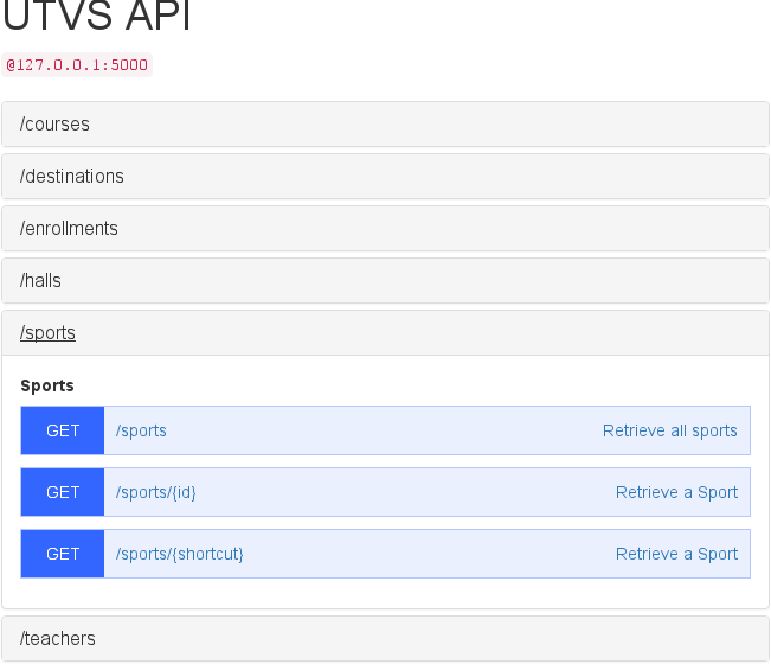
\includegraphics{images/eve-docs}
\caption{Eve: Vygenerovaná HTML dokumentace \label{pic:eve-docs}}
\end{figure}

Generování dokumentace v~Eve je možné s~dalším modulem, systematické a triviální.

\subsection{Funkce služby}\label{funkce-sluux17eby}

\subsubsection*{Stránkování}\label{struxe1nkovuxe1nuxed}

Stránkování se děje automaticky, zobrazenou stránku lze ovlivnit parametrem \verb!page! a počet výsledků na stránce parametrem \verb!max_results!.

\verb!GET /courses/?page=3&max_results=5!

\subsubsection*{Filtrování}\label{filtrovuxe1nuxed}

Filtrovat se dá pomocí JSONu v~parametru \verb!where!. Například takto:

\verb!GET /courses/?where={"teacher": 2}!

Nelze stanovit žádnou podmínku, například větší než apod. Nelze kombinovat více filtrů.

\subsubsection*{Řazení}\label{ux159azenuxed}

Řadit se dá parametrem \verb!sort! podle různých položek a to včetně určení směru řazení a použití více řadících podmínek. Následující příklad seřadí kurzy podle dnu v~týdnu od nejpozdějšího a následně v~případě shody podle čísla haly.

\verb!GET /courses/?sort=-day,hall!

Řazení, filtrování a stránkování se dá libovolně kombinovat.

\subsubsection*{Vyjednávání o~obsahu}\label{vyjednuxe1vuxe1nuxed-o-obsahu}

Na základě hlavičky \emph{Accept} Eve serialuzje do JSONu (výchozí) nebo do XML (\protect\hyperlink{code:eve:xml}{ukázka}).

\verb!GET /courses/1         Accept: application/xml!

\begin{listing}[htbp]
\caption{{\label{code:eve:xml}Eve: Serializace do XML}}
\begin{minted}[bgcolor=codebg]{xml}
<?xml version="1.0"?>
<resource href="courses/1" title="Course">
  <link rel="collection" href="courses" title="courses"/>
  <link rel="hall" href="halls/1" title="Hall"/>
  <link rel="parent" href="/" title="home"/>
  <link rel="sport" href="sports/3" title="Sport"/>
  <link rel="teacher" href="teachers/6" title="Teacher"/>
  <_etag>f27aef6240aecc4ccaaad785dc1bfd89b7a6b889</_etag>
  <day>1</day>
  <ends_at>15:00</ends_at>
  <hall>1</hall>
  <id>1</id>
  <notice/>
  <semester>1</semester>
  <shortcut>BAS01</shortcut>
  <sport>3</sport>
  <starts_at>13:30</starts_at>
  <teacher>6</teacher>
</resource>
\end{minted}
\end{listing}

\subsubsection*{Rozcestník}\label{rozcestnuxedk}

Eve automaticky vytváří rozcestník.

\subsubsection*{Vnořené položky}\label{vnoux159enuxe9-poloux17eky}

Eve umožňuje zobrazit odkazované položky vnořeně, pomocí JSON parametru \verb!embedded!. Toto je potřeba povolit ve schématu (\protect\hyperlink{code:eve:links1}{ukázka}).

\verb!GET /enrollments/28477/?embedded={"course": true}!

\subsection{Další poznámky}\label{dalux161uxed-poznuxe1mky}

Největším problém Eve je absence automaticky vytvořených odkazů a víceméně fixně daný formát výstupu, ten je ale poměrně dobře navržen.

\subsection{Kompletní implementace}\label{kompletnuxed-implementace}

Kompletní implementaci REST API pro rozvrhová data ÚTVS ČVUT ve frameworku Eve najdete na přiloženém médiu a na adrese:

\url{https://github.com/hroncok/utvsapi-eve}
